\section{Astral Symbolism}

\begin{wrapfigure}{rt}{.3\textwidth}
 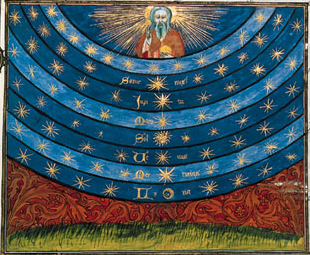
\includegraphics[scale=1.5]{a20220215AstralSymbolism-img001.jpg} 
\end{wrapfigure}

In \emph{Man and his Becoming}, \textbf{Rene Guenon} explains:

\begin{quotex}
Natural phenomena in general, and especially astronomical phenomena, are never looked upon by the traditional doctrines other than as a simple means of expression, whereby they symbolize truths of a higher order.

\end{quotex}
This is true because there is a correspondence between the different degrees. Principles therefore find expression in the human states, as he writes:

\begin{quotex}
If [natural phenomena] symbolize such truths [of a higher order], it is because their laws are fundamentally nothing but the expression of these very truths in a particular domain, a sort of translation of the corresponding principles, naturally adapted to the special conditions of the corporeal and human state.

\end{quotex}
Certainly, this applies a fortiori to astronomical symbolism:

\begin{quotex}
It must be clearly understood, that when mention is made of the Spheres of the Sun and of the Moon, it is never the sun and the moon as visible stars, belonging purely to the corporeal realm, that are referred to, but rather the universal principles which these stars represent after their own fashion in the sensible world … Indeed the different Worlds, planetary Spheres and elementary Realms which are symbolically described as so many regions (only symbolically however, since the being who journeys through them is no longer subject to space), \textbf{are in reality just different states}.

\end{quotex}
Furthermore, as Guenon notes, the same logic applies in the West to the doctrines of Heaven, Hell, and Purgatory. They likewise represent states, not places. Here we have the hermeneutic key to understand Dante's journey. He starts in Hell (the human state), spends time in Purgatory (states of self-purification), and rises to Heaven, passing through all the planetary states.

The same planetary symbolism is also used to represent the chakras. The same understanding applies: the chakras are not physical organs, but represent inner states of the being. Moreover, this understanding is not optional Guenon emphasizes, in regard to these points:

\begin{quotex}
It is absolutely essential for the understanding of these matters.

\end{quotex}
Otherwise, you become like one of:

\begin{quotex}
those who are incapable of understanding anything but the most grossly literal meaning; such people will never realize the workings of a symbol, because their conceptions are irremediably limited to existence on this earth and to the corporeal world, within which, by the most naive of illusions, they wish to imprison the whole of reality.

\end{quotex}
\paragraph{The Literal Meaning}
The symbolic meaning does not debt or replace the literal or historical meaning; rather, the historical event is a consequence of the symbolic or higher meaning. In \emph{The Symbolism of the Cross}, Guenon explains:

\begin{quotex}
The fact is that people too often tend to think that if a symbolical meaning is admitted, the literal or historical sense must be rejected; such a view can only result from unawareness of the \textbf{Law of Correspondence} which is the very foundation of all symbolism. By virtue of this law, each thing, proceeding as it does from a metaphysical principle from which it derives all its reality, translates or expresses that principle in its own fashion and in accordance with its own order of existence, so that from one order to another all things are linked together and correspond in such a way as to contribute to the universal and total harmony, which, in the multiplicity of manifestation, can be likened to a reflection of the principia! unity itself. 

\end{quotex}
To summarize:

\begin{quotex}
The laws of a lower domain can always be taken to symbolize realities of a higher order, wherein resides their own profoundest cause; which is at once their principle and their end. 

\end{quotex}

\hfill

\flrightit{Posted on 2022-02-15 by Cologero }

\begin{center}* * *\end{center}

\begin{footnotesize}\begin{sffamily}



\texttt{TSP on 2022-05-26 at 12:04 said: }

I read something in Guenon's “The Spiritist Fallacy” that has given me serious pause. He denies the astral form and in this he goes against not only Valentin Tomberg, Franz Bardon, the UR Group (see the essay on the “diaphanous body” in “Introduction to Magic Volume II”), but also Fr. Seraphim Rose. In the section “Astral Projection” in “The Soul After Death”, Fr. Rose clearly states that not only is astral projection possible, but that some of the realms one can visit are just as perceptible as our own (which idea is also found in Bardon's work and others). Guenon will have none of this, insisting that the entire notion of the astral plane is a mere caricature and misunderstanding of the subtle state.

I understand that matters such as “astral projection” are of little import as regards the ultimate goal of Gnosis or Moksha; the issue is rather that I can't understand how Guenon could make such a serious error in metaphysics. I am wondering if he ever rectified this elsewhere as he did with regards to his original view of Buddhism, or if he ever at least explained more clearly why he took issue with the idea of the astral form and did not equate it with the soul or subtle body as did Tomberg, Bardon, et al.


\hfill

\texttt{Cologero on 2022-05-27 at 08:28 said: }

You really did your homework, TSP, to get into the weeds like that. Well, you made me look.

I'd prefer to think that G is being overly polemical and his real goal was to move away from the overly materialistic views of those spiritists. It helps a little to compare that text to Man and his Becoming.

G did not deny the subtle states so objections to a “subtle body” or “astral body” seem overly pedantic. In the dream state, they appear as bodies to me, but certainly not as corporeal bodies. I get his point, though. I've heard of experiments that tried to “weigh” the soul as it left the body at death. Such a notion is absurd, although I've known people who believe such things. I believe that is the type of thing Guenon is objecting to.

Obviously, G cannot and does not deny Taijasa, which he discusses on page 97. I think if you read that section, you will find all the phenomena that you mention.


\end{sffamily}\end{footnotesize}
